\documentclass[conference]{IEEEtran}

\usepackage[T1]{fontenc}
\usepackage[utf8]{inputenc}
\usepackage{cite}
\usepackage{url}
\usepackage{booktabs}
\usepackage{array}
\usepackage{tikz}
\usetikzlibrary{arrows.meta, positioning, shapes.geometric}

\title{AI-Enabled Social Media Content Generation and Cross-Platform Scheduling: An IEEE-Style System Study}

\author{
\IEEEauthorblockN{Abhijeet Rai}
\IEEEauthorblockA{
Department of Computer Science and Engineering\\
AI Social Media Automation Agent Project\\
Email: abhijeet1104a@gmail.com
}
}

\begin{document}
\maketitle

\begin{abstract}
Social media publishing increasingly demands rapid ideation, platform-aware wording, and reliable scheduling across professional accounts. This paper presents an AI-enabled social media automation agent designed to assist users in generating captions, connecting social platforms, and publishing posts immediately or at a scheduled time. The system combines a React frontend, FastAPI backend, MongoDB persistence, JWT authentication, OpenAI-based caption generation, OAuth-based account linking, and a worker process that monitors due posts. LinkedIn posting is implemented as the primary publish path, while YouTube, Instagram, and Facebook account-connection flows provide an extensible foundation for later media publishing. The study positions the prototype within recent literature on generative AI marketing, personalization, creativity, misinformation, and human-AI collaboration. System architecture, data collections, endpoint behavior, and scheduling workflow are described through IEEE-style figures and tables. The result is a practical, modular prototype that demonstrates how lightweight AI services can support small teams while preserving human editorial control.
\end{abstract}

\begin{IEEEkeywords}
Generative AI, social media automation, content scheduling, OAuth, FastAPI, React, MongoDB, LinkedIn API, human-AI collaboration.
\end{IEEEkeywords}

\section{Introduction}
Generative artificial intelligence has become a practical tool for marketing communication because it can draft short-form text, summarize campaign ideas, and adapt messages to different audiences. Recent marketing scholarship treats GenAI not only as a productivity tool but also as a technology that changes content design, customer interaction, and organizational innovation \cite{grewal2025,cillo2025,dube2026}. Social media is a natural setting for these capabilities: posts are frequent, time-sensitive, and require variations in tone, hashtags, and platform style. However, useful social media automation is not only a text-generation problem. A deployable system must authenticate users, store content history, manage connected platform accounts, respect platform permissions, and execute scheduled tasks reliably.

This paper presents a system study of an AI social media automation agent developed as a full-stack prototype. The application allows users to sign up, log in, generate social captions from a topic, connect social media accounts through OAuth, publish immediately to LinkedIn, and schedule future posts. The implementation uses a React interface, FastAPI routes, MongoDB Atlas collections, JWT bearer tokens, OpenAI text generation, and a Python worker that checks pending tasks. The backend follows a modular controller-service structure so that platform adapters can be extended without concentrating all behavior in one file.

The paper contributes a concise IEEE-style design analysis rather than a controlled user experiment. It explains the architecture, data model, workflow, and integration challenges involved in building a realistic AI publishing assistant. The discussion also reflects recent concerns about persuasion, misinformation, credibility, and human oversight in AI-mediated content work \cite{matz2024,hoes2024,ahmad2024}. These concerns motivate a human-in-the-loop workflow in which AI drafts are reviewed before posting.

\section{Related Work}
Generative AI is now widely studied in marketing and innovation. Grewal et al. describe how GenAI reshapes marketing practice through customization, human augmentation, and customer interaction \cite{grewal2025}. Cillo and Rubera identify research opportunities across innovation and marketing processes, emphasizing that GenAI can alter idea generation and product communication \cite{cillo2025}. Dubé and Xu provide empirical evidence from email marketing showing that large language models can affect creative content design and business experimentation \cite{dube2026}. Xie et al. analyze the broader AI marketing literature using machine-learning topic modeling, confirming the expanding role of AI in consumer engagement and strategy \cite{xie2025}.

Personalized communication is a second important stream. Chen et al. examine how large language models may transform personalization through conversational and context-aware interaction \cite{chen2024}. Matz et al. show the potential of generative AI for personalized persuasion at scale, which is relevant for social media but also raises ethical concerns \cite{matz2024}. Studies on creativity report that current generative language models can perform strongly on divergent-thinking tasks \cite{hubert2024}, while human-AI collaboration research emphasizes interface design and user self-efficacy \cite{mcguire2024}. These findings support tools where AI assists rather than replaces human judgment.

Social media automation also intersects with risk. Hoes et al. study misinformation interventions and show that corrective strategies can reduce misperceptions while increasing skepticism \cite{hoes2024}. Ahmad et al. highlight how online misinformation may receive advertising support even when consumers object \cite{ahmad2024}. EPJ Data Science studies on social media behavior, credibility inference, and cyber social threats further show why automated publishing tools need accountability and auditability \cite{nwala2023,truong2024,pierri2024,jeon2025}. Consumer response research on human-AI collaboration also warns that audiences may react differently when they know content was AI-assisted \cite{haupt2025}.

\section{System Overview}
The proposed system is a web-based AI assistant for social media content generation, account connection, instant posting, and scheduled posting. Users interact through a React single-page application. The backend exposes authenticated APIs for generation, scheduling, account connection, and post execution. MongoDB stores users, generated content, scheduled posts, connected account tokens, OAuth state values, and logs. The worker process polls scheduled posts every few seconds and executes due items.

\begin{figure}[!t]
\centering
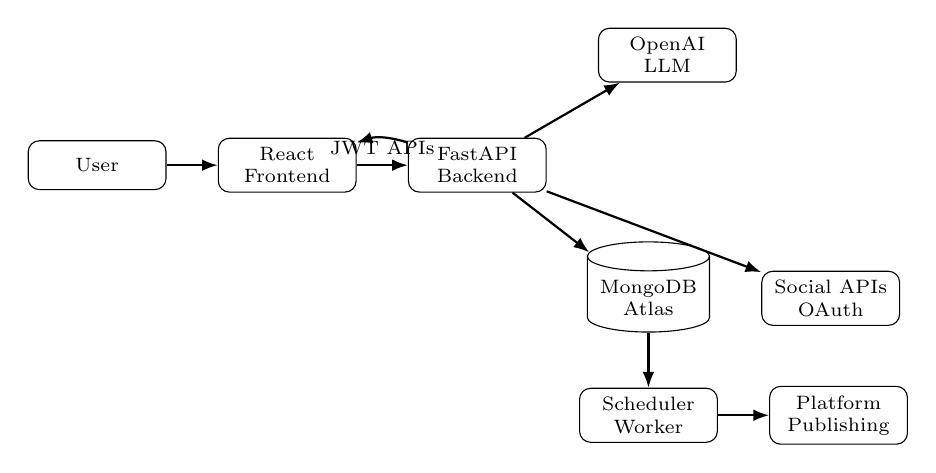
\begin{tikzpicture}[
    node distance=0.70cm and 0.65cm,
    every node/.style={font=\scriptsize},
    box/.style={draw, rounded corners, align=center, minimum width=1.75cm, minimum height=0.62cm},
    db/.style={draw, cylinder, shape border rotate=90, aspect=0.25, align=center, minimum height=0.76cm, minimum width=1.55cm},
    arrow/.style={-{Latex[length=2mm]}, thick}
]
\node[box] (user) {User};
\node[box, right=of user] (react) {React\\Frontend};
\node[box, right=of react] (api) {FastAPI\\Backend};
\node[box, above right=of api] (llm) {OpenAI\\LLM};
\node[db, below right=of api] (mongo) {MongoDB\\Atlas};
\node[box, below=of mongo] (worker) {Scheduler\\Worker};
\node[box, right=of mongo] (oauth) {Social APIs\\OAuth};
\node[box, right=of worker] (publish) {Platform\\Publishing};

\draw[arrow] (user) -- (react);
\draw[arrow] (react) -- node[above] {JWT APIs} (api);
\draw[arrow] (api) -- (llm);
\draw[arrow] (api) -- (mongo);
\draw[arrow] (api) -- (oauth);
\draw[arrow] (mongo) -- (worker);
\draw[arrow] (worker) -- (publish);
\draw[arrow] (api) to[bend right=18] (react);
\end{tikzpicture}
\caption{Architecture of the AI-enabled social media automation agent.}
\label{fig:architecture}
\end{figure}

The account-connection module supports LinkedIn, YouTube, Instagram, and Facebook through platform-specific OAuth routes. LinkedIn is the primary implemented publishing path because the application can use the \texttt{w\_member\_social} permission after the user reconnects with that scope. YouTube upload and Instagram/Facebook publishing require additional media and platform-policy handling, so their current implementation focuses on account connection and token storage.

\section{Methodology}
\subsection{Application Design}
The backend was refactored into a lightweight model-view-controller style organization. Controllers define route behavior, services encapsulate social-platform API logic, configuration reads environment variables, and the database module centralizes MongoDB collections. This separation reduces accidental coupling between authentication, generation, scheduling, and OAuth code.

\begin{table}[!t]
\centering
\caption{Main Backend Modules}
\label{tab:modules}
\begin{tabular}{p{2.5cm}p{5.2cm}}
\toprule
\textbf{Module} & \textbf{Responsibility}\\
\midrule
\texttt{main.py} & FastAPI app setup, CORS, router registration\\
\texttt{controllers} & Authentication, posts, account connection, system routes\\
\texttt{services} & LinkedIn, YouTube, Instagram, and Facebook API logic\\
\texttt{auth.py} & Password hashing, JWT creation, token verification\\
\texttt{database.py} & MongoDB client and collection references\\
\texttt{worker.py} & Polling scheduled posts and executing due publishing tasks\\
\bottomrule
\end{tabular}
\end{table}

\subsection{Workflow}
The content workflow has two paths. In the instant path, a user generates a caption, clicks ``Post Now,'' and the backend publishes the content through the connected LinkedIn account. In the scheduled path, the user selects date and time; the backend stores a pending record; the worker later finds the due record and publishes it.

\begin{figure}[!t]
\centering
\begin{tikzpicture}[
    node distance=0.55cm,
    every node/.style={font=\scriptsize},
    step/.style={draw, rounded corners, align=center, minimum width=5.4cm, minimum height=0.55cm},
    arrow/.style={-{Latex[length=2mm]}, thick}
]
\node[step] (a) {User enters topic and requests AI caption};
\node[step, below=of a] (b) {Backend calls LLM and stores generated draft};
\node[step, below=of b] (c) {User selects Post Now or Schedule};
\node[step, below=of c] (d) {Backend checks connected account and platform scope};
\node[step, below=of d] (e) {Immediate publish or pending schedule record};
\node[step, below=of e] (f) {Worker publishes due posts and updates status};
\draw[arrow] (a) -- (b);
\draw[arrow] (b) -- (c);
\draw[arrow] (c) -- (d);
\draw[arrow] (d) -- (e);
\draw[arrow] (e) -- (f);
\end{tikzpicture}
\caption{Generation, posting, and scheduling workflow.}
\label{fig:workflow}
\end{figure}

\subsection{Data Model}
The database uses separate collections for users, generated posts, scheduled posts, connected accounts, OAuth state, and logs. This design allows user-specific filtering, platform-specific tokens, and audit records to be queried independently.

\begin{table}[!t]
\centering
\caption{Core MongoDB Collections}
\label{tab:collections}
\begin{tabular}{p{2.6cm}p{5.1cm}}
\toprule
\textbf{Collection} & \textbf{Stored Data}\\
\midrule
\texttt{users} & Username and bcrypt-hashed password\\
\texttt{posts} & Generated draft content, topic, owner, timestamp\\
\texttt{scheduled\_posts} & Content, date, time, platforms, status, publish results\\
\texttt{connected\_accounts} & OAuth tokens, scopes, profile data, platform metadata\\
\texttt{oauth\_states} & Temporary state values for callback validation\\
\texttt{logs} & Worker success and failure records\\
\bottomrule
\end{tabular}
\end{table}

\section{Implementation}
The frontend is implemented with React components for authentication, content generation, account connection, recent posts, dashboard display, and footer support. The account modal uses dropdown panels so that each social account opens only when selected. When a platform is connected, the panel shows profile information, scopes, an open-account action, and a logout action. This reduces visual clutter and gives users clearer control over connected platforms.

The backend uses FastAPI with JWT bearer authentication. Environment variables store API keys, OAuth client credentials, redirect URLs, and scopes. OAuth flows are separated per platform. The LinkedIn service builds the authorization URL, exchanges authorization codes, retrieves user information, stores tokens, and publishes text posts. YouTube, Instagram, and Facebook services follow the same account-connection pattern, although full publishing support depends on platform permissions and media constraints.

The scheduler worker checks pending posts and attempts publication when the scheduled time is within a short execution window. On success, it marks the record as posted and stores platform result identifiers. On failure, it increments retry count and eventually marks the post as failed. This approach is simple but adequate for a prototype; production systems would replace polling with a durable queue, distributed locks, and observability tooling.

\section{Results and Discussion}
The resulting prototype demonstrates that a small web application can combine content generation, account management, and automated publishing without requiring a monolithic backend file. The controller-service split makes platform expansion straightforward: each new platform mainly requires a service module, routes for OAuth, and a frontend dropdown panel. The system also shows why real posting is harder than draft generation. Social platforms require different OAuth scopes, redirect URL policies, app review processes, and publishing endpoints. For example, LinkedIn text posting requires a posting permission, YouTube uploads require upload scope and media transfer handling, and Facebook Page posting may require Meta review.

From a human-centered perspective, the prototype keeps users in the loop. AI drafts are not automatically published; a user chooses whether to post immediately or schedule. This design aligns with research showing both the creative potential of LLMs and the need for human oversight \cite{hubert2024,mcguire2024}. It also reduces risk in a domain where persuasive communication and misinformation can have social consequences \cite{matz2024,hoes2024,ahmad2024}. However, the current prototype still needs content safety checks, factuality warnings, rate-limit handling, media upload workflows, and formal user testing.

\section{Limitations}
The study is limited to a system prototype and does not include a controlled evaluation of user productivity, caption quality, or engagement outcomes. Platform publishing is uneven because each API has different review and permission requirements. LinkedIn text posting is the clearest path, while YouTube, Instagram, and Facebook require further work for media upload and Page/Business approval. The scheduler also uses polling rather than a production-grade queue. Finally, no automated plagiarism or AI-detection claim is made; originality depends on responsible writing, citation, and review.

\section{Conclusion}
This paper presented an IEEE-style system study of an AI-enabled social media automation agent. The prototype integrates React, FastAPI, MongoDB, JWT authentication, OpenAI-based caption generation, OAuth account connection, immediate posting, and scheduled publishing through a worker process. Its modular backend separates controllers, services, configuration, authentication, and database access, making the project easier to extend than a single-file implementation. LinkedIn is implemented as the primary text-publishing channel, while YouTube, Instagram, and Facebook account flows establish a path toward broader platform support once required permissions and media workflows are complete.

The work shows that practical social media automation requires more than prompt engineering. Account authorization, token storage, platform scopes, retry behavior, recent-post visibility, and user-facing feedback are equally important. The design therefore preserves human control: AI generates drafts, but users decide whether to post immediately or schedule for later. This is important because recent studies show that generative AI can support creativity and personalization, while also creating risks related to persuasion, credibility, and misinformation. Future work should add media upload pipelines, safety filters, factuality checks, analytics dashboards, queue-based scheduling, role-based access control, and user studies comparing manual and AI-assisted workflows. A later evaluation could measure drafting time, user satisfaction, posting reliability, and perceived authenticity across connected platforms. With these improvements, the system can become a more robust tool for small teams that need efficient yet accountable social media operations.

\begin{thebibliography}{00}

\bibitem{grewal2025}
D. Grewal, C. B. Satornino, T. Davenport, and A. Guha, ``How generative AI is shaping the future of marketing,'' \emph{Journal of the Academy of Marketing Science}, vol. 53, pp. 702--722, 2025, doi: 10.1007/s11747-024-01064-3.

\bibitem{cillo2025}
P. Cillo and G. Rubera, ``Generative AI in innovation and marketing processes: A roadmap of research opportunities,'' \emph{Journal of the Academy of Marketing Science}, vol. 53, pp. 684--701, 2025, doi: 10.1007/s11747-024-01044-7.

\bibitem{dube2026}
J.-P. Dubé and A. Xu, ``Large language models and creative content design: A case study of email marketing at Wine Access,'' \emph{Quantitative Marketing and Economics}, vol. 24, no. 1, 2026, doi: 10.1007/s11129-025-09303-9.

\bibitem{xie2025}
H. Xie, Y. Nie, L. Liu, and Y. Chen, ``Machine learning-based research of AI marketing: Topic analysis and model construction,'' \emph{Future Business Journal}, vol. 11, no. 272, 2025, doi: 10.1186/s43093-025-00686-5.

\bibitem{chen2024}
J. Chen \emph{et al.}, ``When large language models meet personalization: Perspectives of challenges and opportunities,'' \emph{World Wide Web}, vol. 27, no. 42, 2024, doi: 10.1007/s11280-024-01276-1.

\bibitem{matz2024}
S. C. Matz \emph{et al.}, ``The potential of generative AI for personalized persuasion at scale,'' \emph{Scientific Reports}, vol. 14, no. 4692, 2024, doi: 10.1038/s41598-024-53755-0.

\bibitem{hubert2024}
K. F. Hubert, K. N. Awa, and D. L. Zabelina, ``The current state of artificial intelligence generative language models is more creative than humans on divergent thinking tasks,'' \emph{Scientific Reports}, vol. 14, no. 3440, 2024, doi: 10.1038/s41598-024-53303-w.

\bibitem{mcguire2024}
J. McGuire, D. De Cremer, and T. Van de Cruys, ``Establishing the importance of co-creation and self-efficacy in creative collaboration with artificial intelligence,'' \emph{Scientific Reports}, vol. 14, no. 18525, 2024, doi: 10.1038/s41598-024-69423-2.

\bibitem{hoes2024}
E. Hoes \emph{et al.}, ``Prominent misinformation interventions reduce misperceptions but increase scepticism,'' \emph{Nature Human Behaviour}, vol. 8, pp. 1545--1553, 2024, doi: 10.1038/s41562-024-01884-x.

\bibitem{ahmad2024}
W. Ahmad \emph{et al.}, ``Companies inadvertently fund online misinformation despite consumer backlash,'' \emph{Nature}, vol. 630, pp. 123--131, 2024, doi: 10.1038/s41586-024-07404-1.

\bibitem{nwala2023}
A. C. Nwala, A. Flammini, and F. Menczer, ``A language framework for modeling social media account behavior,'' \emph{EPJ Data Science}, vol. 12, no. 33, 2023, doi: 10.1140/epjds/s13688-023-00410-9.

\bibitem{truong2024}
B. T. Truong, O. M. Allen, and F. Menczer, ``Account credibility inference based on news-sharing networks,'' \emph{EPJ Data Science}, vol. 13, no. 10, 2024, doi: 10.1140/epjds/s13688-024-00450-9.

\bibitem{pierri2024}
F. Pierri \emph{et al.}, ``Computational approaches for cyber social threats,'' \emph{EPJ Data Science}, vol. 13, no. 65, 2024, doi: 10.1140/epjds/s13688-024-00504-y.

\bibitem{jeon2025}
M. S. Jeon \emph{et al.}, ``Simulating conversations on social media with generative agent-based models,'' \emph{EPJ Data Science}, vol. 14, no. 79, 2025, doi: 10.1140/epjds/s13688-025-00593-3.

\bibitem{haupt2025}
M. Haupt, J. Freidank, and A. Haas, ``Consumer responses to human-AI collaboration at organizational frontlines: Strategies to escape algorithm aversion in content creation,'' \emph{Review of Managerial Science}, vol. 19, pp. 377--413, 2025, doi: 10.1007/s11846-024-00748-y.

\end{thebibliography}

\end{document}
